A continuación se detallará la estructura completa del gestor de contenidos.  Como se ha explicado en la sección ``\nameref{chapter02:alternativas_seleccionadas}'' perteneciente al capítulo \ref{chapter02}, el gestor de contenidos seleccionado ha sido Drupal.


\subsubsection{Diagrama de componentes}
La figura \ref{fig:diagrama_componentes_cms} muestra el diagrama de los componentes que forman parte del gestor de contenidos.
\begin{landscape}
	\begin{figure}[ht]
		\centering
		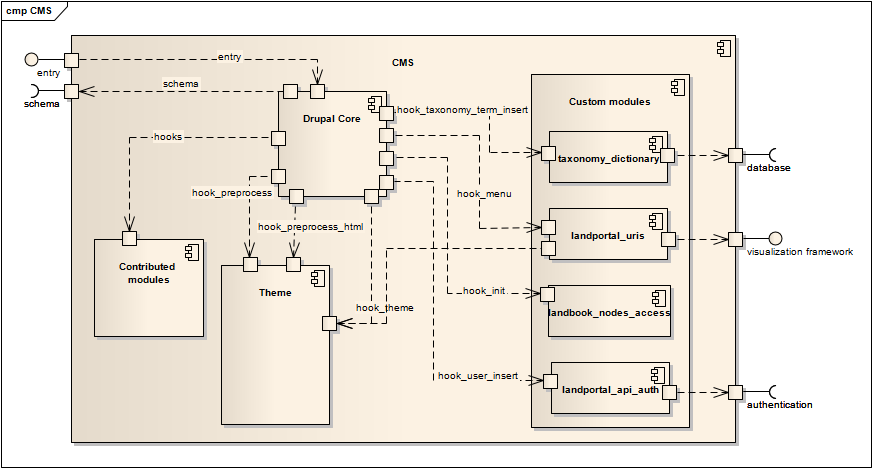
\includegraphics[height=\textwidth]{arquitectura/cms_view}
		\caption{Diagrama de componentes del gestor de contenidos}
		\label{fig:diagrama_componentes_cms}
	\end{figure}
\end{landscape}


\subsubsection{Descripción de los componentes}
Se describirán ahora los distintos componentes que forman parte del gestor de contenidos. La organización de dichos componentes puede verse en la figura \ref{fig:diagrama_componentes_cms}
\begin{description}
	\item[Drupal Core]  El núcleo de Drupal implementa la funcionalidad principal del gestor de contenidos.  Es el encargado de procesar y responder a las peticiones, además de coordinar el funcionamiento de los diferentes módulos y temas visuales.
	\item[Contributed modules]  Los módulos contribuidos son módulos realizados por terceros y que han sido públicamente incluidos en el repositorio de módulos de Drupal.  Éstos módulos amplían la funcionalidad existente en el núcleo de Drupal\footnote{Actualmente existen unos 15.000 módulos que forman parte del repositorio.  Dichos módulos pueden verse en \url{https://www.drupal.org/project/project_module}}.
	\item[Custom modules]  Los módulos propios han sido especialmente creados para éste proyecto y realizan alguna funcionalidad que no forma parte del núcleo de Drupal ni de ningún módulo contribuido.  Se han desarrollado cuatro módulos propios:
		\begin{itemize}
			\item \textit{taxonomy\_dictionary}  Permite relacionar los datos existentes en la base de datos con los términos de las taxonomías existentes en Drupal.
			\item \textit{landportal\_uris}  Implementa un sistema similar al MVC para facilitar la creación de vistas.  También incluye el framework que provee de datos a las visualizaciones.  Éste módulo se verá con más detalle posteriormente en la sección ``\nameref{vista_landportal_uris}'' de éste mismo capítulo.
			\item \textit{landbook\_nodes\_access}  Permite redirigir a las vistas adecuadas cuando se visite alguno de los nodos de la sección de datos.
			\item \textit{landportal\_api\_auth}  Genera y almacena las claves de autenticación del el API para los nuevos usuarios que se creen en el sistema.
		\end{itemize}
	\item[Theme]  El tema implementa la interfaz de las diferentes vistas que forman parte del gestor de contenidos.
\end{description}


\subsubsection{Relación entre los componentes}
Las peticiones entrantes son procesadas por el núcleo de Drupal.  En cada petición el núcleo de Drupal invoca los módulos que estén suscritos a los \textit{hooks} adecuados para que realicen su funcionalidad\footnote{El módulo ``\textit{landportal\_uris}'' será detallado posteriormente en la sección ``\nameref{vista_landportal_uris}'' de éste mismo capítulo.  El resto de módulos propios cuentan simplemente con un único fichero que implementa el \textit{hook} correspondiente por lo que, dada su sencillez, sus vistas se omitirán}:
\begin{itemize}
	\item Cuando se crea un nuevo término en la taxonomía se invoca al módulo \textit{taxonomy\_dictionary} para que lo enlace con el término correspondiente en la base de datos.
	\item Cuando se realiza una petición que no va dirigida a mostrar la vista de administración se invoca al módulo \textit{landportal\_uris} para que provea los datos con los que se renderizarán posteriormente las vistas del tema.
	\item Cuando se accede a alguno de los nodos pertenecientes a la zona de datos se invoca al módulo \textit{landbook\_nodes\_access} para que realice la redirección hacia la vista adecuada.
	\item Cuando se crea un nuevo usuario en el portal se invoca al módulo \textit{landportal\_api\_auth} para que cree y almacene sus claves de acceso al API.
\end{itemize}
Por último, el núcleo de Drupal invoca al tema para que renderice las vistas que serán mostradas al usuario que realiza la petición.


\subsubsection{Interfaces y puertos}
A continuación se detallarán las interfaces y puertos de los componentes que forman parte del gestor de contenidos. 

\paragraph{CMS} \hfill \\
La tabla \ref{interfaces_cms_cms} muestra el detalle de las interfaces del \textit{CMS}.

\begin{longtable}[c]{|p{25mm}|p{20mm}|p{30mm}|p{60mm}|}
 \caption{Vista del gestor de contenidos - interfaces del \textit{CMS}.\label{interfaces_cms_cms}}\\

 %Cabecera en la primera pagina
 \hline
 	Interfaz & Tipo & Tecnología & Propiedades\\
 \hline
 \hline
 \endfirsthead
 %Cabecera en el resto de páginas
 \hline
 \multicolumn{4}{|c|}{Continuación de la tabla \ref{interfaces_receiver_receiver}}\\
 \hline
 	Interfaz & Tipo & Tecnología & Propiedades\\
 \hline
 \hline
 \endhead
 %Tabla
 \hline
 \endfoot
 
	\textbf{entry} & Proveída & Petición HTTP & Recibe las peticiones procedentes del exterior \\
	\hline
		
	\textbf{schema} & Requerida & API del motor de búsqueda & Envía los datos del gestor de contenidos al motor de búsqueda para su indexación\footnote{ Como se ha explicado en la sección ``\nameref{chapter02:alternativas_seleccionadas}'' perteneciente al capítulo \ref{chapter02}, el motor de búsqueda seleccionado ha sido \textit{Apache Solr}} \\
	\hline
	
	\textbf{database} & Requerida & Conexión a base de datos & Accede a la base de datos donde se almacena la información perteneciente al subsistema de datos \\
	\hline
	
	\textbf{visualization framework} & Proveída & API Web & Provee datos con los que posteriormente crear las visualizaciones\footnote{Los elementos de éste framework podrán ser vistos con mayor detalle posteriormente en la sección ``\nameref{vista_landportal_uris}'' perteneciente a éste mismo capítulo} \\
	\hline
	
	\textbf{authentication} & Proveída & API REST & Genera claves de autenticación en el API para los usuarios del portal \\
\hline
\hline

 \end{longtable}


\paragraph{Drupal Core} \hfill \\
La tabla \ref{interfaces_cms_drupalcore} muestra el detalle de las interfaces del \textit{núcleo de Drupal}.  

\begin{longtable}[c]{|p{25mm}|p{20mm}|p{30mm}|p{60mm}|}
	\caption{Vista del gestor de contenidos - interfaces del \textit{núcleo de Drupal}.\label{interfaces_cms_drupalcore}}\\
	%Cabecera en la primera pagina
		\hline
			Interfaz & Tipo & Tecnología & Propiedades\\
		\hline
		\hline
	\endfirsthead
	%Cabecera en el resto de páginas
		\hline
		\multicolumn{4}{|c|}{Continuación de la tabla \ref{interfaces_cms_drupalcore}}\\
		\hline
			Interfaz & Tipo & Tecnología & Propiedades\\
		\hline
		\hline
	\endhead
	%Tabla
	\hline
	\endfoot
		\textbf{entry} & Puerto de entrada & Petición HTTP & Recibe las peticiones procedentes del exterior \\
		\hline
		
		\textbf{schema} & Puerto de salida & API del motor de búsqueda & Envía los datos del gestor de contenidos al motor de búsqueda para su indexación \\
		\hline
		
		\textbf{hooks} & Puerto de salida & Llamada a método & Invoca a los módulos que estén suscritos al \textit{hook} correspondiente \\
		\hline
		
		\textbf{hook preprocess} & Puerto de salida & Llamada a método & Indica al tema que preprocese las variables que sean necesarias para las vistas \\
		\hline
		
		\textbf{hook preprocess html} & Puerto de salida & Llamada a método & Indica al tema que preprocese las variables que sean necesarias para la plantilla HTML \\
		\hline
		
		\textbf{hook theme} & Puerto de salida & Llamada a método & Indica al tema que renderice una determinada plantilla para una vista \\
		\hline
		
		\textbf{hook taxonomy term insert} & Puerto de salida & Llamada a método & Indica a un módulo que se ha creado un nuevo término en la taxonomía para que éste realice su funcionalidad \\
		\hline
		
		\textbf{hook menu} & Puerto de salida & Llamada a método & Permite a un módulo registrar rutas para definir cómo son atendidas las peticiones HTTP \\
		\hline
		
		\textbf{hook init} & Puerto de salida & Llamada a método & Indica a un módulo que acaba de tener lugar una petición por parte de un usuario \\
		\hline
		
		\textbf{hook user insert} & Puerto de salida & Llamada a método & Indica a un módulo que acaba de producirse el registro de un nuevo usuario \\
	\hline
	\hline
\end{longtable}


\paragraph{Contributed modules} \hfill \\
La tabla \ref{interfaces_cms_modules} muestra el detalle de las interfaces de los \textit{módulos contribuidos}.  

\begin{longtable}[c]{|p{25mm}|p{20mm}|p{30mm}|p{60mm}|}
	\caption{Vista del gestor de contenidos - interfaces de los \textit{módulos contribuidos}.\label{interfaces_cms_modules}}\\
	%Cabecera en la primera pagina
		\hline
			Interfaz & Tipo & Tecnología & Propiedades\\
		\hline
		\hline
	\endfirsthead
	%Cabecera en el resto de páginas
		\hline
		\multicolumn{4}{|c|}{Continuación de la tabla \ref{interfaces_cms_modules}}\\
		\hline
			Interfaz & Tipo & Tecnología & Propiedades\\
		\hline
		\hline
	\endhead
	%Tabla
	\hline
	\endfoot
		\textbf{hooks} & Puerto de entrada & Llamada a método & Invocados por el núcleo de Drupal cuando tienen lugar ciertos eventos en el sistema \\
	\hline
	\hline
\end{longtable}


\paragraph{Theme} \hfill \\
La tabla \ref{interfaces_cms_theme} muestra el detalle de las interfaces del \textit{tema}.  

\begin{longtable}[c]{|p{25mm}|p{20mm}|p{30mm}|p{60mm}|}
	\caption{Vista del gestor de contenidos - interfaces del \textit{tema}.\label{interfaces_cms_theme}}\\
	%Cabecera en la primera pagina
		\hline
			Interfaz & Tipo & Tecnología & Propiedades\\
		\hline
		\hline
	\endfirsthead
	%Cabecera en el resto de páginas
		\hline
		\multicolumn{4}{|c|}{Continuación de la tabla \ref{interfaces_cms_theme}}\\
		\hline
			Interfaz & Tipo & Tecnología & Propiedades\\
		\hline
		\hline
	\endhead
	%Tabla
	\hline
	\endfoot
		\textbf{hook preprocess} & Puerto de entrada & Llamada a método & Preprocesa las variables que sean necesarias para la posterior renderización de las vistas \\
		\hline
			
		\textbf{hook preprocess html} & Puerto de entrada & Llamada a método & Preprocesa las variables necesarias para renderizar la plantilla HTML \\
		\hline
			
		\textbf{hook theme} & Puerto de entrada & Llamada a método & Renderiza la plantilla de una determinada vista \\
	\hline
	\hline
\end{longtable}


\paragraph{Taxonomy dictionary} \hfill \\
La tabla \ref{interfaces_cms_taxonomy_dictionary} muestra el detalle de las interfaces del módulo ``\textit{Taxonomy dictionary}''.  

\begin{longtable}[c]{|p{25mm}|p{20mm}|p{30mm}|p{60mm}|}
	\caption{Vista del gestor de contenidos - interfaces del módulo \textit{Taxonomy dictionary}. \label{interfaces_cms_taxonomy_dictionary}}\\
	%Cabecera en la primera pagina
		\hline
			Interfaz & Tipo & Tecnología & Propiedades\\
		\hline
		\hline
	\endfirsthead
	%Cabecera en el resto de páginas
		\hline
		\multicolumn{4}{|c|}{Continuación de la tabla \ref{interfaces_cms_taxonomy_dictionary}}\\
		\hline
			Interfaz & Tipo & Tecnología & Propiedades\\
		\hline
		\hline
	\endhead
	%Tabla
	\hline
	\endfoot
		\textbf{hook taxonomy term insert} & Puerto de entrada & Llamada a método & Recibe la información de un nuevo término que se ha creado en la taxonomía \\
		\hline
		\textbf{database} & Puerto de salida & Conexión a base de datos & Almacena la información del término insertado en la taxonomía en la entrada correspondiente de la base de datos \\
	\hline
	\hline
\end{longtable}


\paragraph{LandPortal URIs} \hfill \\
La tabla \ref{interfaces_cms_landportal_uris} muestra el detalle de las interfaces del módulo ``\textit{LandPortal URIs}''.  

\begin{longtable}[c]{|p{25mm}|p{20mm}|p{30mm}|p{60mm}|}
	\caption{Vista del gestor de contenidos - interfaces del módulo \textit{LandPortal URIs}. \label{interfaces_cms_landportal_uris}}\\
	%Cabecera en la primera pagina
		\hline
			Interfaz & Tipo & Tecnología & Propiedades\\
		\hline
		\hline
	\endfirsthead
	%Cabecera en el resto de páginas
		\hline
		\multicolumn{4}{|c|}{Continuación de la tabla \ref{interfaces_cms_landportal_uris}}\\
		\hline
			Interfaz & Tipo & Tecnología & Propiedades\\
		\hline
		\hline
	\endhead
	%Tabla
	\hline
	\endfoot
		\textbf{hook menu} & Puerto de entrada & Llamada a método & El gestor de contenidos está definiendo las rutas que tendrán las vistas del portal \\
		\hline
		\textbf{hook theme} & Puerto de salida & Llamada a método & Indica al tema que renderice una determinada plantilla para una vista \\
		\hline
		\textbf{visualization framework} & Puerto de salida & API Web & Provee datos con los que posteriormente crear las visualizaciones \\
		\hline
		\textbf{database} & Puerto de salida & Conexión a base de datos & Obtiene información de la base de datos \\
	\hline
	\hline
\end{longtable}


\paragraph{LandbBook nodes access} \hfill \\
La tabla \ref{interfaces_cms_landbook_nodes_access} muestra el detalle de las interfaces del módulo ``\textit{LandbBook nodes access}''.  

\begin{longtable}[c]{|p{25mm}|p{20mm}|p{30mm}|p{60mm}|}
	\caption{Vista del gestor de contenidos - interfaces del módulo \textit{LandbBook nodes access}. \label{interfaces_cms_landbook_nodes_access}}\\
	%Cabecera en la primera pagina
		\hline
			Interfaz & Tipo & Tecnología & Propiedades\\
		\hline
		\hline
	\endfirsthead
	%Cabecera en el resto de páginas
		\hline
		\multicolumn{4}{|c|}{Continuación de la tabla \ref{interfaces_cms_landbook_nodes_access}}\\
		\hline
			Interfaz & Tipo & Tecnología & Propiedades\\
		\hline
		\hline
	\endhead
	%Tabla
	\hline
	\endfoot
		\textbf{hook init} & Puerto de entrada & Llamada a método & Invocada por el núcleo del gestor de contenidos cuando acaba de tener lugar una petición por parte de un usuario \\
	\hline
	\hline
\end{longtable}


\paragraph{Landportal API auth} \hfill \\
La tabla \ref{interfaces_cms_landportal_api_auth} muestra el detalle de las interfaces del módulo ``\textit{LandPortal API auth}''.  

\begin{longtable}[c]{|p{25mm}|p{20mm}|p{30mm}|p{60mm}|}
	\caption{Vista del gestor de contenidos - interfaces del módulo \textit{LandPortal API auth}. \label{interfaces_cms_landportal_api_auth}}\\
	%Cabecera en la primera pagina
		\hline
			Interfaz & Tipo & Tecnología & Propiedades\\
		\hline
		\hline
	\endfirsthead
	%Cabecera en el resto de páginas
		\hline
		\multicolumn{4}{|c|}{Continuación de la tabla \ref{interfaces_cms_landportal_api_auth}}\\
		\hline
			Interfaz & Tipo & Tecnología & Propiedades\\
		\hline
		\hline
	\endhead
	%Tabla
	\hline
	\endfoot
		\textbf{hook user insert} & Puerto de entrada & Llamada a método & Invocado por el núcleo del gestor de contenidos cuando se realiza el registro de un nuevo usuario \\
		\hline
		\textbf{authentication} & Puerto de salida & API REST & Genera claves de autenticación en el API para el usuario recién registrado en el portal \\
	\hline
	\hline
\end{longtable}
